\chapter{Development and Testing}
\label{chap:development}

\section{Introduction to Development Approach}
The development approach in this chapter is informed by modern software engineering practices and recent advances in real-time system development \cite{cantelon2017nodejs,tilkov2018nodejs,li2020realtime,blogmicro2023}.
\lipsum[1]

\subsection{Overview of the Development Methodology}
The iterative methodology adopted here is consistent with recommendations from \cite{fowler2015microservices,kleppmann2013designing,rauch2022scalable}.
\lipsum[2]
\begin{itemize}
    \item \textbf{Iterative Delivery:} Features are developed in small increments.
    \item \textbf{Continuous Feedback:} Regular reviews and stakeholder input.
    \item \textbf{Quality Focus:} Automated tests and code reviews.
\end{itemize}
The project adopted a modern, iterative development methodology to ensure rapid delivery of features, continuous feedback, and adaptability to changing requirements. Emphasis was placed on code quality, automation, and collaboration among team members.

\subsection{Agile Workflow and Iteration Cycles}
\lipsum[3]
\begin{itemize}
    \item \textbf{Sprint Planning:} Define goals and tasks for each cycle.
    \item \textbf{Daily Stand-ups:} Synchronize team progress.
    \item \textbf{Retrospectives:} Reflect and improve process.
\end{itemize}
Development was organized into short sprints, each focused on delivering a set of prioritized features or improvements. Daily stand-ups, sprint planning, and retrospectives were used to maintain alignment and address blockers promptly.

\subsection{Task Management and Version Control Practices}
\lipsum[4]
\begin{itemize}
    \item \textbf{Branching Strategy:} Feature, develop, and release branches.
    \item \textbf{Pull Requests:} Peer review and automated checks.
    \item \textbf{Issue Tracking:} Use of labels, milestones, and boards.
\end{itemize}
Tasks were tracked using GitHub Issues and project boards. All code changes were managed via Git and GitHub, with feature branches, pull requests, and code reviews enforced to maintain code quality and traceability.

\section{Development Environment and Tools}
\lipsum[5]

\subsection{Programming Languages, Frameworks, and Libraries}
The choice of programming languages and frameworks is based on their suitability for scalable, event-driven applications, as discussed in \cite{cantelon2017nodejs,brown2019websockets,nodejsdocs,blogkafka2022}.
\lipsum[6]
\begin{itemize}
    \item \textbf{Node.js:} Main runtime for backend services.
    \item \textbf{WebSocket Libraries:} ws, uWebSockets.js, Socket.IO.
    \item \textbf{Supporting Libraries:} Express, dotenv, Winston, etc.
\end{itemize}

\subsection{Comparison of WebSocket Libraries}
Table~\ref{tab:websocket-comparison} compares the main WebSocket libraries considered for this project.
\begin{table}[H]
    \centering
    \caption{Comparison of WebSocket Libraries}
    \label{tab:websocket-comparison}
    \begin{tabularx}{\textwidth}{l c X X}
        \toprule
        \textbf{Library} & \textbf{Performance} & \textbf{Feature Set} & \textbf{Ease of Use} \\
        \midrule
        ws & High & Basic WebSocket functionality with minimal protocol overhead & Simple low-level API suitable for custom implementations \\
        uWebSockets.js & Very High & Advanced HTTP and WebSocket support implemented on a C++ core & More complex API but delivers the highest performance \\
        Socket.IO & Moderate & Rich feature set including rooms, fallback transports, and events & High-level abstraction that is easy to use but less efficient \\
        \bottomrule
    \end{tabularx}
\end{table}
\textbf{Library selection:} \texttt{ws} was chosen for its balance of performance, simplicity, and ecosystem support. \texttt{uWebSockets.js} offers the highest performance but is less mature and harder to debug. \texttt{Socket.IO} provides many features but adds protocol overhead and is less efficient for raw real-time messaging.


\subsection{Development Environment Setup}
\lipsum[7]
\begin{figure}[H]
    \centering
    % Replace with your environment setup diagram
    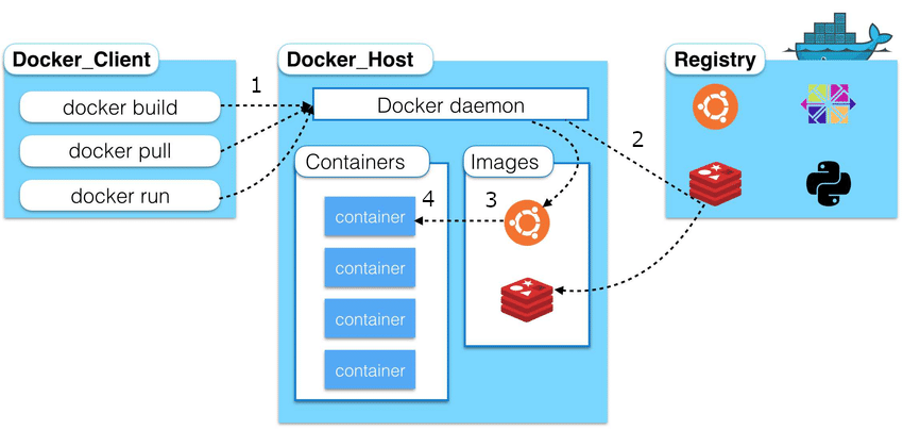
\includegraphics[width=0.7\textwidth]{images/dev-env.png}
    \caption{Local development environment setup.}
    \label{fig:dev-env}
\end{figure}
A local development stack was provisioned using Docker Compose, enabling rapid onboarding and consistent environments. Environment variables and runtime configuration files were used to manage secrets and deployment-specific settings.

\subsection{Supporting Tools}
\lipsum[8]
A suite of supporting tools was used to streamline development:
\begin{itemize}
    \item \textbf{Git/GitHub:} Source control and collaboration
    \item \textbf{Postman / Insomnia:} API testing and documentation
    \item \textbf{Docker / Docker Compose:} Containerized development and deployment
    \item \textbf{ESLint, Prettier:} Code linting and formatting
\end{itemize}

\section{Source Code Structure and Module Organization}
\lipsum[9]

\subsection{Project Directory Structure}
\lipsum[10]
\begin{figure}[H]
    \centering
    % Replace with your directory structure diagram
    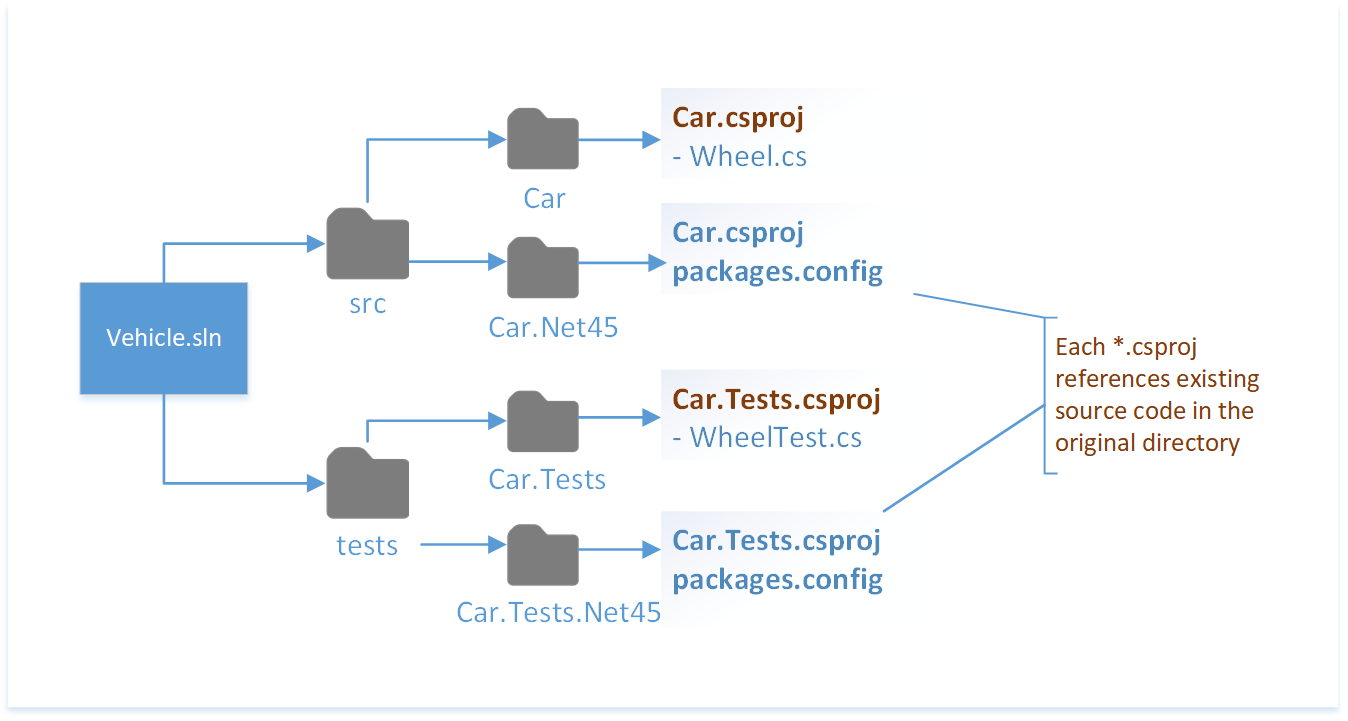
\includegraphics[width=0.8\textwidth]{images/project-structure.png}
    \caption{Project directory structure.}
    \label{fig:project-structure}
\end{figure}
The project directory was organized to separate concerns and promote maintainability. Key folders included \texttt{src/}, \texttt{config/}, \texttt{tests/}, and \texttt{docker/}.

\subsection{Core Modules}
\lipsum[11]
The codebase was modularized into the following core components:
\begin{itemize}
    \item \textbf{Gateway module:} Implements the WebSocket server and manages client connections
    \item \textbf{Messaging module:} Handles publish/subscribe logic and message routing
    \item \textbf{Channel management module:} Manages channels, memberships, and permissions
    \item \textbf{Persistence module:} Interfaces with the database and storage systems
    \item \textbf{Authentication module:} Manages user authentication and authorization
\end{itemize}

\subsection{Code Conventions and Naming Standards}
\lipsum[12]
\begin{itemize}
    \item \textbf{CamelCase:} For variables and function names.
    \item \textbf{PascalCase:} For class and component names.
    \item \textbf{UPPERCASE:} For constants and environment variables.
\end{itemize}
Consistent code conventions and naming standards were enforced throughout the project, following widely accepted JavaScript/TypeScript best practices.

\subsection{Configuration and Secrets Management}
\lipsum[13]
Sensitive configuration values and secrets were managed using environment variables and secure vaults, never hardcoded in the source code.


\section{Implementation of Core Features}

\subsection{Sample Code Snippets for Core Modules}

\paragraph{Gateway Module (WebSocket Server)}
This snippet illustrates a minimal WebSocket gateway implemented using the \texttt{ws} library. 
The gateway is responsible for accepting client connections, performing authentication, and handling incoming real-time messages.

\begin{lstlisting}[language=JavaScript, caption={Minimal WebSocket Gateway using ws}]
const WebSocket = require('ws');
const wss = new WebSocket.Server({ port: 8080 });
wss.on('connection', (ws, req) => {
    // Authenticate user from token in req
    ws.on('message', (msg) => {
        // Handle incoming message
    });
});
\end{lstlisting}

\paragraph{Pub/Sub Module (Redis Example)}
The following example demonstrates how Redis Pub/Sub is used to broadcast messages to multiple connected clients. 
This mechanism enables horizontal scalability by decoupling message producers from consumers.

\begin{lstlisting}[language=JavaScript, caption={Redis Pub/Sub for message fan-out}]
const redis = require('redis');
const pub = redis.createClient();
const sub = redis.createClient();
sub.subscribe('messages');
sub.on('message', (channel, message) => {
    // Deliver message to connected clients
});
// To publish:
pub.publish('messages', JSON.stringify({ ... }));
\end{lstlisting}

\paragraph{Persistence Module (MongoDB Example)}
This code snippet shows how chat messages are persisted to a MongoDB database. 
Storing messages in a document-oriented database ensures durability and supports efficient retrieval for chat history.

\begin{lstlisting}[language=JavaScript, caption={Persisting a message to MongoDB}]
const { MongoClient } = require('mongodb');
const client = new MongoClient(uri);
await client.connect();
const db = client.db('chat');
await db.collection('messages').insertOne({ sender, content, timestamp });
\end{lstlisting}

\subsection{WebSocket Connection Lifecycle}
\lipsum[15]
The connection lifecycle includes the initial handshake, session initialization, and robust auto-reconnect logic to ensure reliability.
\begin{itemize}
    \item \textbf{Handshake process:} Secure upgrade from HTTP(S) to WebSocket
    \item \textbf{Session initialization:} User authentication and session state setup
    \item \textbf{Auto-reconnect behavior:} Exponential backoff and session resumption
\end{itemize}

\subsection{Message Send/Receive Pipeline}
\lipsum[16]
The message pipeline validates incoming messages, persists them, and efficiently delivers them to all intended recipients using a fan-out strategy.
\begin{itemize}
    \item \textbf{Validation:} Schema and permission checks
    \item \textbf{Persistence:} Durable storage in the database
    \item \textbf{Delivery FAN-OUT logic:} Efficient broadcast to channel members
\end{itemize}

\subsection{Presence Tracking Implementation}
\lipsum[17]
Presence is tracked in real time using in-memory data stores (e.g., Redis) and periodic heartbeats from clients.

\subsection{Typing Indicator Implementation}
\lipsum[18]
Typing indicators are implemented using throttled WebSocket events, providing real-time feedback to channel participants.

\subsection{Read Receipts and Delivery Status}
\lipsum[19]
Read receipts and delivery status are managed by tracking per-user message offsets and updating clients in real time.

\subsection{Rate Limiting and Flood Protection}
\lipsum[20]
Rate limiting is enforced at the gateway and messaging layers to prevent abuse, using token bucket algorithms and per-user quotas.

\subsection{Logging, Monitoring, and Metrics Integration}
\lipsum[21]
\begin{table}[H]
    \centering
    \caption{Sample metrics collected in the system.}
    \label{tab:metrics}
    \begin{tabular}{ll}
        \toprule
        \textbf{Metric} & \textbf{Description} \\
        \midrule
        Active Connections & Number of open WebSocket connections \\
        Message Throughput & Messages processed per second \\
        Error Rate & Number of failed operations \\
        Latency (P95) & 95th percentile message delivery latency \\
        \bottomrule
    \end{tabular}
\end{table}
Comprehensive logging and metrics are integrated using tools like Winston, Prometheus, and Grafana for observability and troubleshooting.

\section{Deployment Setup}
\lipsum[22]

\subsection{Local Deployment with Docker}
\lipsum[23]
Developers can spin up the entire stack locally using Docker Compose, which orchestrates all required services and dependencies.

\subsection{Production Deployment Workflow}
\lipsum[24]
Production deployments follow a blue-green or rolling update strategy, with automated health checks and rollback mechanisms.

\subsection{Continuous Integration and Delivery Pipeline (CI/CD)}
\lipsum[25]
CI/CD pipelines are implemented using GitHub Actions, automating build, test, and deployment steps for every code change.

\subsection{Load Balancer \& Reverse Proxy Configuration}
\lipsum[26]
Nginx or HAProxy is configured as a reverse proxy and load balancer, handling TLS termination and distributing traffic to backend nodes.


\section{Testing Strategy}
The testing strategy for this project draws on best practices from both academic and industry sources \cite{guth2018comparison,kim2023iot,nguyen2021pubsub,blogmicro2023}.

\subsection{Detailed Testing Process}
\paragraph{Sample Test Case (Jest)}
\begin{lstlisting}[language=JavaScript, caption={Sample unit test for message validation}]
const validateMessage = require('../src/validateMessage');
test('rejects empty message', () => {
    expect(() => validateMessage('')).toThrow();
});
\end{lstlisting}

\paragraph{Test Coverage}
Test coverage is measured using Istanbul/nyc. Coverage reports are generated on every CI run, and minimum thresholds are enforced (e.g., 90\% statements, 85\% branches).

\paragraph{CI/CD Pipeline Illustration}
\begin{figure}[H]
        \centering
        %\includegraphics[width=0.7\textwidth]{images/cicd-pipeline.png}
        \caption{CI/CD pipeline: build, test, coverage, deploy}
        \label{fig:cicd-pipeline}
\end{figure}
The CI/CD pipeline (implemented with GitHub Actions) automatically builds, tests, checks coverage, and deploys the application on every push or pull request. Failed tests or insufficient coverage block deployment.

\subsection{Overview of Testing Levels}
\lipsum[28]
Testing is performed at multiple levels to ensure correctness and reliability:
\begin{itemize}
    \item \textbf{Unit Testing:} Isolates and tests individual functions and modules
    \item \textbf{Integration Testing:} Validates interactions between components
    \item \textbf{End-to-End (E2E) Testing:} Simulates real user scenarios across the full stack
\end{itemize}

\subsection{Test Tooling}
\lipsum[29]
\begin{itemize}
    \item \textbf{Jest:} Unit and integration testing.
    \item \textbf{Mocha:} Flexible test runner for Node.js.
    \item \textbf{Supertest:} HTTP assertions for REST APIs.
    \item \textbf{Artillery, k6:} Load and performance testing.
\end{itemize}
Popular tools such as Jest, Mocha, Supertest, Artillery, and k6 are used for various testing needs, from unit to load testing.

\subsection{Code Coverage Metrics}
\lipsum[30]
Code coverage is tracked using Istanbul/nyc, with thresholds enforced in CI to maintain high test quality.

\subsection{Test Data Management}
\lipsum[31]
Test data is managed using fixtures and factories, ensuring repeatable and isolated test runs.

\section{Automated Testing}
\lipsum[32]

\subsection{CI/CD Integration}
\lipsum[33]
Automated tests are run on every pull request and push to main branches, ensuring regressions are caught early.

\subsection{Automated Unit Tests}
\lipsum[34]
Unit tests are written for all core modules, with mocks and stubs used to isolate dependencies.

\subsection{Automated Integration Tests}
\lipsum[35]
Integration tests validate end-to-end flows, including WebSocket and REST API interactions.

\subsection{WebSocket Event Simulation Scripts}
\lipsum[36]
Custom scripts simulate WebSocket events and user behavior to test real-time features under various scenarios.

\section{Performance and Load Testing}

% Performance and load testing, as well as experimental results, are presented in detail in Chapter~\ref{chap:deployment} (Deployment and Evaluation).

\section{Scalability Testing}
\lipsum[42]

\subsection{Horizontal Scaling Tests}
\lipsum[43]
Tests are conducted to verify that the system scales linearly with the addition of nodes and resources.

\subsection{Distributed Pub/Sub Load Testing}
\lipsum[44]
The pub/sub layer is stress-tested for message delivery consistency and latency across distributed nodes.

\subsection{Multi-node Messaging Consistency Testing}
\lipsum[45]
Consistency of message delivery and ordering is validated in multi-node deployments.

\subsection{Failover and Recovery Testing}
\lipsum[46]
Simulated node failures and network partitions are used to test the system's ability to recover and maintain service continuity.

\section{Security Testing}
Security testing is guided by established standards and recent research on secure messaging systems \cite{roberts2020aws,awsdocs,zhang2021aws,redisdocs}.
\lipsum[47]

\subsection{Authentication/Authorization Tests}
\lipsum[48]
Tests verify that only authorized users can access protected resources and perform privileged actions.

\subsection{WebSocket Security Tests}
\lipsum[49]
\begin{itemize}
    \item \textbf{Flooding:} Simulate excessive connection and message attempts
    \item \textbf{Replay attacks:} Attempt to reuse old messages or tokens
    \item \textbf{Message spoofing:} Test for unauthorized message injection
\end{itemize}

\subsection{Penetration Testing Overview}
\lipsum[50]
Penetration tests are conducted to identify vulnerabilities and validate the effectiveness of security controls.

\subsection{OWASP-Based Test Checklist}
\lipsum[51]
A checklist based on the OWASP Top 10 is used to ensure comprehensive coverage of common web and API security risks.

\section{Summary of Development and Testing}
\lipsum[52]

This chapter has summarized the development methodology, environment, implementation, deployment, and testing strategies for the real-time messaging system. Major milestones and test results have been highlighted, along with identified gaps and recommendations for future improvements.
